\section{Lecture 25: Interior point methods}
In last lecture, we discussed Newton's method. Although it enjoyes a fast local
convergence guarantee, global convergence of Newton's method is not guaranteed. 
In this lecture, we'll introduce interior point methods, which can be thought of
as an extension of Newton's method to ensure global convergence.  We will first
introduce the main idea of \emph{barrier methods} at great generality, before we
specialize our analysis to linear pogramming.

\subsection{Barrier methods}
Barrier methods replace inequality constraints with a so-called \emph{barrier}
function that is added to objective function of the optimization problem. 
Consider the following optimization problem: 
\begin{align*}
\min_x  &\quad f(x)\\
\text{s.t.} &\quad x\in{\domain},\\
&\quad g_j(x)\leqslant{0}\,,\qquad j=1,2,\cdots,r\,,
\end{align*}
where $f:\R^n\rightarrow\R$, $g_j:\R^n\rightarrow\R$ are given functions. 
The function~$f$ is continuous, and $\domain$ is a closed set. For the rest of the lecture, we assume convex $g_j$ and $\domain=\R^n$. And we denote $x^*$ as the optimal solution of the problem.

\begin{definition}[Interior of the constraint region]
The interior (relative to $\domain$) of the constraint region is defined as $S=\{x\in\domain:g_j(x)<0,\ j=1,2,\cdots,r\}$. 
\end{definition}

Assuming nonempty and convex $S$, we define a so-called barrier function $B(x)$
defined on $S$, such that $B(x)$ is continuous the function blows up as we
approach the boundary of the constraint region. More formally,
$\lim_{g_j(x)\rightarrow{0_{\_}}}B(x)=\infty$. Two most common examples are
logarithmic barrier function and inverse barrier function: 
\begin{align}
\text{Logarithmic:}\qquad B(x) &= -\sum_{j=1}^{r}\ln\{-g_j(x)\}\\
\text{Inverse:}\qquad B(x) &= -\sum_{j=1}^{r}\frac{1}{g_j(x)}.
\end{align}
Both of them are convex if all $g_j(x)$ are convex. 

\begin{figure}[ht]
\centering
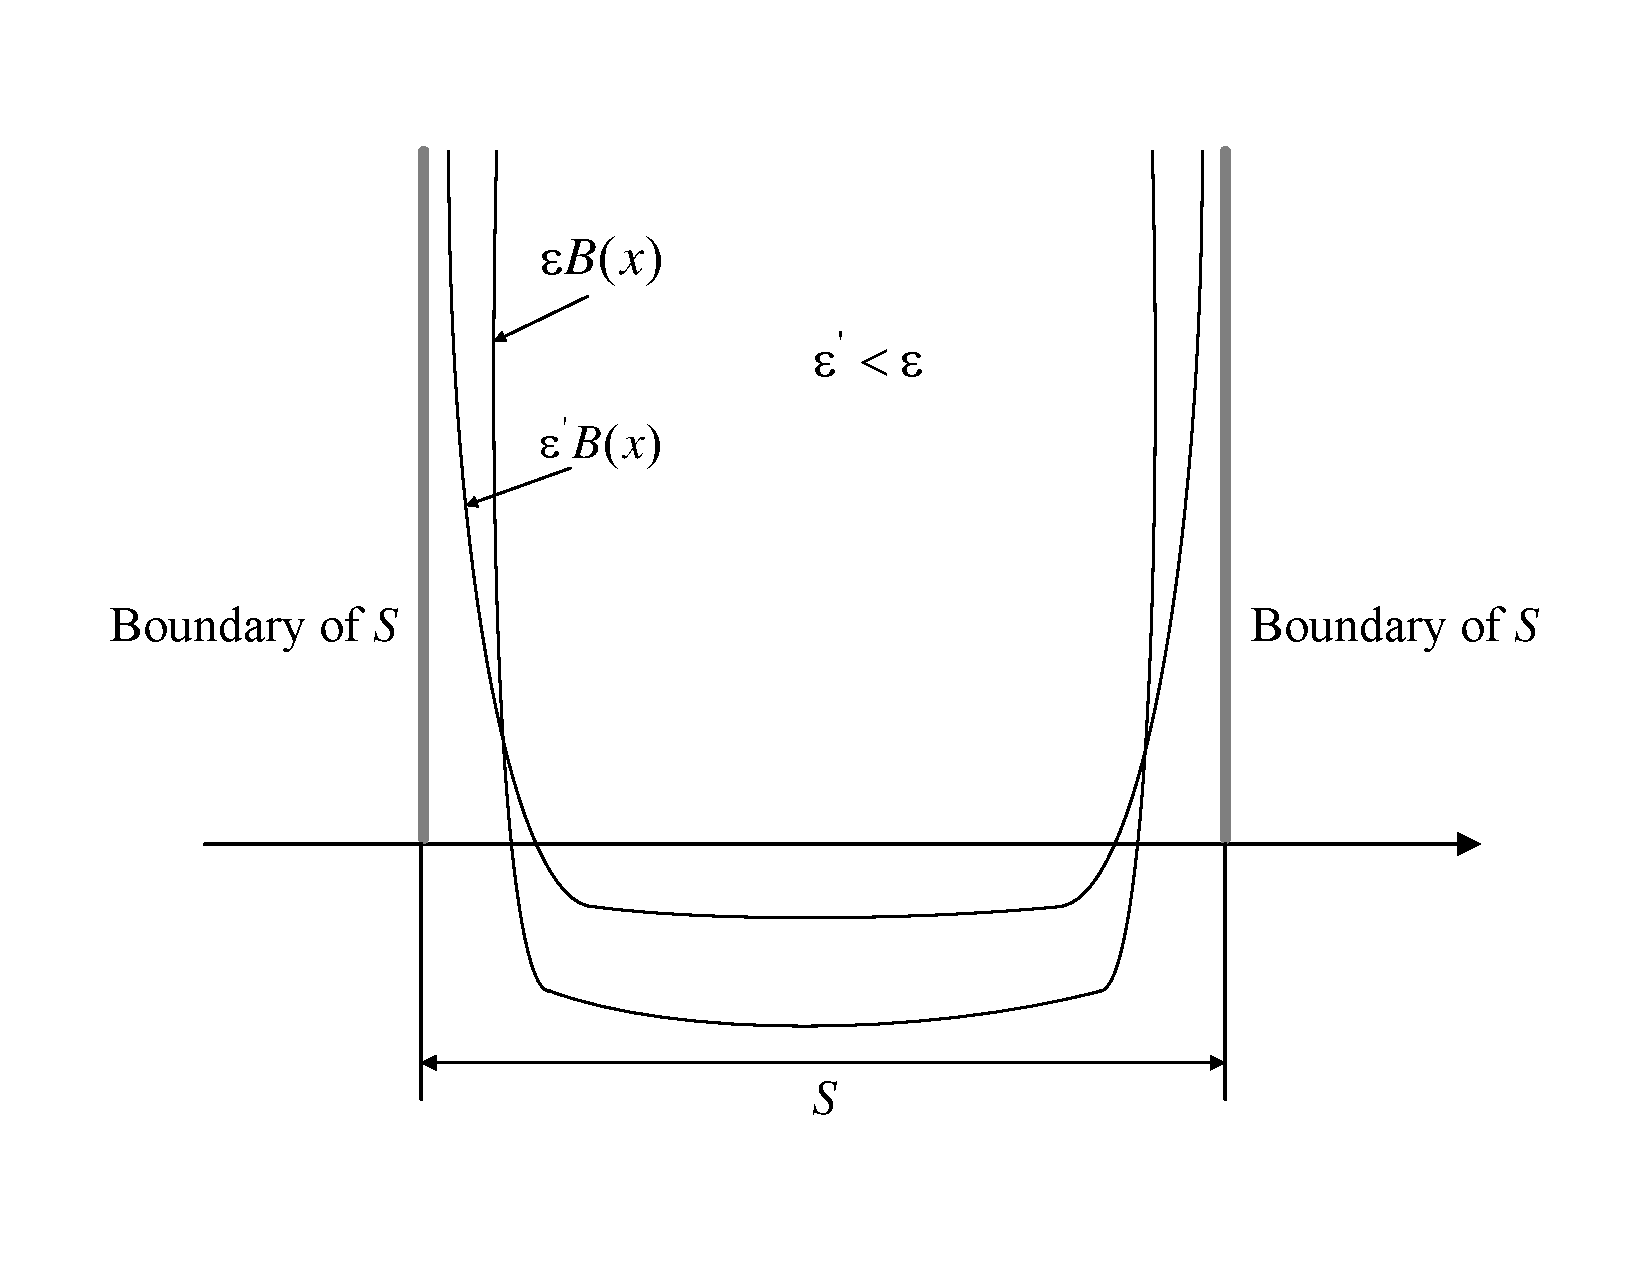
\includegraphics[scale=0.4]{figures/lecture25-barrier_function}
\caption{Form of a barrier term}
\label{fig:barrier}
\end{figure}

Given a barrier function $B(x)$, define a new cost function
$f_\epsilon(x)=f(x)+\epsilon{B(x)}$, where $\epsilon$ is a positive real number.
Then we can eliminate the inequality constraints in the original problem and
obtain the following problem: 
%
\begin{equation}
\begin{aligned}
&\min_x & {f_\epsilon(x)}\\
&\qquad\text{s.t.} & x\in{\domain},\\
\end{aligned}
\end{equation}
The form of the barrier term $\epsilon{B(x)}$ is illustrated in Figure \ref{fig:barrier}.

The barrier method is defined by introducing a sequence $\{\epsilon_t\}$ such
that $0<\epsilon_{t+1}<\epsilon_t$ for $t=0,1,2,...$ and
$\epsilon_t\rightarrow{0}$. Then we find a sequence $\{x_t\}$ such that
$x_t\in{\arg \min_{x\in{S}}}f_{\epsilon_t}(x)$. Note that the barrier term
$\epsilon_t{B(x)}$ goes to zero for all interior points $x\in{S}$ as
$\epsilon_t\rightarrow{0}$, allowing $x_t$ to get increasingly closer to the
boundary. Therefore, intuitively, $x_t$ should approach $x^*$ no matter $x^*$ is
in the interior or on the boundary of $S$. Its convergence is formalized in the
following proposition. 

\begin{proposition}
Every limit point of a sequence $\{x_t\}$ generated by a barrier method is a global minimum of the original constrained problem. 
\end{proposition}
\begin{proof}
See Proposition 5.1.1 of \cite{bertsekas2016nonlinear}.
\end{proof}

As $\domain=\R^n$, Newton's method can be applied with properly selected
stepsize to ensure that all iterates lies in $S$. Concretely, an initial
interior point can be obtained for some large $\epsilon_0$. Then in each
iteration, we can use $x_t$ as an initialization to find $x_{t+1}$ by Newton's
method. When $\epsilon_0$ is large, it is easier to find a interior point. And
since $x_t$ is close to $x_{t+1}$, it is likely that $x_t$ is in the local
convergence region for Newton's method. Therefore, intuitively, global
convergence of Newton's method can be enabled by using barrier methods.

\subsection{Linear programming}

We'll now adopt the logarithmic barrier method to solve the linear programming (LP) problem defined as follows:
\begin{equation}
\label{eq:LP_def}
\text{LP}:\qquad
\begin{aligned}[c|c|c]
&\min_x &c^\trans&x\\
&\qquad\text{s.t.} &Ax&\ge b
\end{aligned}
\end{equation}
where $A\in{\R}^{m\times n}$ with $m\ge n$ and $\mathrm{rank}(A)=n$. Denote $x^*$ as the optimal point. 

First we write out the augmented cost function by the logarithmic barrier method, i.e.,
\begin{equation}
\label{eq:LP_aug_cost}
f_\epsilon(x) = c^\trans x-\epsilon \sum_{j=1}^m\ln\left(A^\trans_j x-b\right).
\end{equation}
where $A^\trans_j$ is the $j$-th row of $A$. Define $x^*_\epsilon=\argmin_x f_\epsilon(x)$. 

\begin{fact}
The optimal point $x^*_\epsilon$ exists and is unique for any $\epsilon>0$.
\end{fact}
\begin{proof}
We can easily check that $f_\epsilon(x)$ is convex (as a sum of two convex functions). Therefore, the minimizer $x^*_\epsilon$ must exist and is unique.

To show the convexity of $f_\epsilon$, we can check the second-order derivative,
which is positive definite as shown in \eqref{eq:hessian_f_eps} later.
\end{proof}

\subsubsection{Central path}
The central path of the LP problem in \ref{eq:LP_def} is depicted by the set of
$\left\{x^*_\epsilon|\epsilon>0\right\}$, as shown in \figureref{fig:central_path}.
\begin{figure}[h!]
\centering
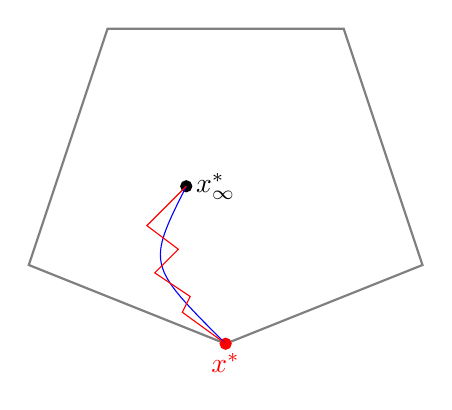
\begin{tikzpicture}
\draw[gray, thick] (-1,2) -- (2,2) -- (3,-1) -- (0.5,-2) -- (-2,-1) -- cycle;
\filldraw[black] (0,0) circle (2pt) node[anchor=west] {$x^*_\infty$};
\filldraw[red] (0.5,-2) circle (2pt) node[anchor=north] {$x^*$};
\draw[blue, thin] (0,0) .. controls (-0.5,-1) .. (0.5,-2);
\draw[red, thin] (0,0) -- (-0.5,-0.5) -- (-0.1,-0.8) -- (-0.4,-1.1) -- (0.05,-1.4) -- (-0.05,-1.6) -- (0.5,-2);
\end{tikzpicture}
\caption{The central path\label{fig:central_path}}
\end{figure}

Our goal is to design an algorithm that will approximately follow the central
path. Assume that we already have a ``good enough'' initial point, then at every step, we apply one step of Newton's method. To guarantee that the algorithm converges, we need to answer the following two questions:
\begin{itemize}
\item Under what conditions does the single-step Newton method work?
\item How should we update $\epsilon$?
\end{itemize}

\subsubsection{Newton Decrement}
To apply Newton's method, first we need to find out the first-order and second-order derivatives of $f_\epsilon$. Note that
\begin{eqnarray}
\nabla f_\epsilon(x)&=&c-\epsilon \sum_{j=1}^m \dfrac{A_j}{A^\trans_j x-b}\triangleq c-\epsilon A^\trans S^{-1}\mathbb{1}\label{eq:grad_f_eps}\\
\nabla^2f_\epsilon(x)&=&\epsilon A^\trans S^{-2}A=\epsilon \sum_{j=1}^m\dfrac{A_j A_j^\trans}{S_j^2}\label{eq:hessian_f_eps}
\end{eqnarray}
where $\mathbb{1}=[1,1,\cdots,1]^\trans\in\mathbb{R}^{m\times1}$, $S=\mathrm{diag}\{A^\trans_1 x-b, A^\trans_2 x-b, \cdots, A^\trans_m x-b\}$.

Then the Newton update can be applied:
\begin{equation}
\bar{x}=x-[\nabla^2f_\epsilon(x)]^{-1}\nabla f_\epsilon(x)=x-[\epsilon A^\trans S^{-2}A]^{-1}\left(c-\epsilon A^\trans S^{-1}\mathbb{1}\right)\label{eq:Newton_update}
\end{equation}

Recall that Newton's method finds the solution by making the first-order condition zero. To measure how much the Newton update will decrease the first-order approximation, we introduce the concept of Newton decrement.

Define the Newton decrement as
\begin{equation}
q^2(x, \epsilon) = \nabla f_\epsilon(x)^\trans[\nabla^2f_\epsilon(x)]^{-1}\nabla f_\epsilon(x)\label{eq:newton_decrement}
\end{equation}
or $q(x, \epsilon) = \left\|[\nabla^2f_\epsilon(x)]^{-1/2}\nabla f_\epsilon(x)\right\|_2$. 

Note that the Newton decrement also relates to the difference between $f_\epsilon(x)$ and the minimum of its second-order approximation:
\begin{eqnarray}
&&f_\epsilon(x)-\min_{\bar{x}}\left(f_\epsilon(x)+\nabla f_\epsilon(x)^\trans(\bar{x}-x)+(\bar{x}-x)^\trans\nabla^2 f_\epsilon(x)(\bar{x}-x)\right)\nonumber\\
&=&f_\epsilon(x)-\left(f_\epsilon(x)-\dfrac{1}{2}\nabla f_\epsilon(x)^\trans[\nabla^2f_\epsilon(x)]^{-1}\nabla f_\epsilon(x)\right)\nonumber\\
&=&\dfrac{1}{2}\nabla f_\epsilon(x)^\trans[\nabla^2f_\epsilon(x)]^{-1}\nabla f_\epsilon(x)\triangleq \dfrac{1}{2}q^2(x, \epsilon).
\end{eqnarray}

We'll then use Newton decrement to find out the conditions for convergence
guarantee of the algorithm. 

\subsubsection{An update rule and its convergence guarantee}
We'll now come up with an update rule that can guarantee convergence if some initial conditions are satisfied. To develop the update rule, we first introduce the following propositions. 
\begin{proposition}\label{prop1}
Assume $Ax > b$ and $q(x, \epsilon)<1$, then we have
\begin{align}
c^\trans x-c^\trans x^{*}\leq 2\epsilon n.
\end{align}
\end{proposition}
In particular, if we maintain that $x_t$ is interior point satisfying $Ax_t>b$,
and $q(x_t, \epsilon_t) < 1$, then $c^\trans x_t$ converges to $c^\trans x^*$ as $\epsilon_t$ goes to $0$, i.e., $x_t$ converges to global optimum. However, the condition $q(x_t,\epsilon_t)<1$ is not trivial.  

\begin{proposition}\label{prop2}
If $Ax>b$, and $q(x,\epsilon)<1$, then the pure Newton iterate
step $\bar{x}$ satisfies,
\begin{align}
q(\bar{x}, \epsilon) &\leq q(x, \epsilon)^2 
\end{align}
\end{proposition}
It ensures that $q(\bar{x}, {\epsilon})<1$ given $q(x,\epsilon)<1$ and $x$ is interior point. But we also want that $q(\bar{x}, \bar{\epsilon})<1$ for some $\bar{\epsilon}<\epsilon$. 

\begin{proposition}\label{prop3}
Assume $q(x,\epsilon)\leq \frac{1}{2}$, interior point $Ax>b$,
put 
\begin{align}
\bar{\epsilon} = \left(1-\frac{1}{6\sqrt{n}}\right)\epsilon,
\end{align}
then we have
\begin{align}
q(\bar{x}, \bar{\epsilon})\leq \frac{1}{2}
\end{align}
\end{proposition}
These propositions suggest the following update rule,
\begin{align}
x_{t+1} & = x_t - \nabla^2 f_{\epsilon_t}(x)^{-1}\nabla f_{\epsilon_t}(x_t) \\
\epsilon_t & = \left(1-\frac{1}{6\sqrt{n}}\right)\epsilon
\end{align}
\begin{theorem}
Suppose $(x_0, \epsilon_0)$ satisfies $Ax_0 >b$ and 
$q(x_0,\epsilon_0)\leq\frac{1}{2}$, then the algorithm
converges in $\mathcal{O}(\sqrt{n}\log(n/\eta))$ iterations to $\eta$ error, i.e., we have $c^\trans x_t\leqslant{c^\trans x^*+\eta}$ after $\mathcal{O}(\sqrt{n}\log(n/\eta))$ iterations.
\end{theorem}

\begin{proof}
As Newton step maintains $x_{t+1}$ in the interior, by using the three propositions above, we have 
\begin{eqnarray}
c^\trans x_t&\leqslant&{c^\trans x^*+2\epsilon_t{n}}\nonumber\\
&=&{c^\trans x^*+2\left(1-\frac{1}{6\sqrt{n}}\right)^t\epsilon_0}\nonumber\\
&\leqslant&{c^\trans x^*+2\exp\left(-\frac{t}{6\sqrt{n}}\right)\epsilon_0}
\end{eqnarray}
Therefore, to have a error of $\eta$, $t\geqslant{\frac{6\sqrt{n}}{\epsilon_0}}\log{\frac{2n}{\eta}}$. We can then conclude that the algorithm converges in  $\mathcal{O}(\sqrt{n}\log(n/\eta))$ iterations to $\eta$ error. 
\end{proof}

The algorithm stated above is the so-called short-step method. Although theoretical convergence rate is guaranteed, the combination of small decrease in $\epsilon$ and a single Newton step is slow in practice. Instead, a more practical method is the so-called long-step method, where $\epsilon$ is reduced in faster rate and several Newton steps are taken per iteration.
